\chapter[A Flow Approach for Data Delivery Optimization]{$\mathit{DynFloR}$: A Flow Approach for Data Delivery Optimization in Multi-Robot Network Patrolling}
\label{flow}

Deploying fleets of mobile robots in real scenarios and environments raises several scientific challenges. One of them concerns the ability of the robots to adapt to the dynamics of their environment. We introduce $\mathit{DynFloR}$ \cite{kes}, a dynamic network flow based approach for finding optimal policies for \emph{data delivery} in \emph{multi-robot network patrolling} where the robots can communicate instantly and free of charge one to another, there is a periodicity of the robot meetings and the distribution of the data collected during the patrol is regular. Experiments on randomly generated synthetic examples are performed for evaluating the performance of the $\mathit{DynFloR}$ method. The performed experiments empirically show that independent of the problem setting (such as number of robots, memory of the robots) the amount of data transferred to a base station per unit of time converges to an equilibrium state. The case of lost data has been also examined through various experiments, but it requires further experimentation as well as in-depth analysis. This chapter represents the first step in a research which is being conducted for using \emph{reinforcement learning} in order to optimize data delivery in a general multi-robot network patrolling case, when the patrolling environment is non-deterministic and uncertain.

The study performed  in this chapter represents the starting point of a broader research which is being conducted for optimizing data delivery in DMRP using \emph{reinforcement learning} (RL) \cite{AsisHHS18}, in the more general case when there is an uncertainty in the environment (i.e. there is no periodicity in the robots' meetings). In this general case, the robots will have to learn through \emph{reinforcement} (RL) \cite{Konidaris12} the data transfer policy, in order to maximize the quantity of transmitted data.
 
The contribution of this chapter consists in a new approach, $DynFloR$, based on dynamic network flows for determining the optimal policy for delivering data in multi-robot network patrolling under the following assumptions: the environment is deterministic, the network of robots is centralized and offline and the robots have periodic meetings. The proposed $DynFloR$ method adapts the approach proposed by  Kotnyek \cite{flow} for the problem of MRP. It can be also extended for the DMRP under the previously mentioned assumptions. We assume the data transfer to be dynamic and we address the following research question: \emph{How to optimize data-passing between each robot cycle in order to maximize the quantity of data transmitted to the sink?} Experiments and simulations performed on several synthetic and randomly generated examples emphasize that our proposal is able to determine a policy that maximizes the data transferred to the base station up to a given moment in time.  The answer to the previously stated RQ through the $DynFloR$ approach will provide us additional insights on the nondeterministic MRP/DMRP problem and its modelling as a reinforcement learning task. To the best of our knowledge, $DynFloR$ approach is new in the MRP literature.

The rest of the chapter is structured as follows.  Our $DynFloR$ approach for data delivery optimization in a deterministic setting of the MRP is introduced in Section \ref{our}. Section \ref{discussion} presents the experimental results obtained by evaluating $DynFloR$ and provides a comparison to existing similar approaches. Furthermore, in Section \ref{discussion} we have a discussion about the current solution as well as its advantages and limitations. Section \ref{conc} contains the conclusions of the chapter and directions to continue our research.

\section{Methodology}\label{our}

This section introduces our centralized and offline $DynFloR$ approach for data delivery optimization in a deterministic setting of the MRP. $DynFloR$ is  applicable in a deterministic setting of DMRP, as well. 

\subsection{Problem definition. Theoretical model}\label{tm}

The problem we are approaching in this chapter is defined in the following. We assume the particular case of a deterministic environment, in which the network of robots is centralized and offline:  \emph{There are $n$ robots, which can meet and exchange data. The robots are continuously collecting data on the cycles they patrol. There are initial meeting times for the robots and meeting periods. The goal is to maximize the quantity of data arriving to a sink (a base station) in a given time T}.

Let us consider the following theoretical model.  We denote by $\mathcal{R}=\{R_1, R_2, \cdots, R_n\}$ the set of patrolling robots. We assume the sink is denoted by $R_0$. Each robot $R_i \in \mathcal{R}$ patrols a certain cycle $C_i$ consisting of $k_i$ targets, i.e. $C_i=\{t_i^{1}, t_i^{2}, \dots t_i^{k_i}\}$. At each visit of the target $t_i^{j}$, an amount $d_i^{j}$ of data  will be collected by robot $R_i$. Hence, after patrolling a complete cycle, robot $R_i$ collects a quantity of data  $D_i=\displaystyle \sum_{j=1}^{k_i}{d_i^{j}}$. This data is stored in robot $R_i$'s memory, of maximum capacity $\mathit{MaxCapacity_i}$.  We consider that the sink has no memory limit, i.e. $MaxCapacity_0=\infty$. For data exchange, two robots $R_i$ and $R_j$ have periodical meetings (\emph{rendez-vous} points) starting at time  $T_{ij}$ when they first meet, with a period of $\pi_{ij}$ time steps.   

In our approach, we assume that the incoming data model is \emph{regular} and \emph{known} and that there is a single base station (called {\em sink}). The data is continuously collected by the robots after patrolling their cycle and has to be transmitted to the sink. We also assume that it takes one unit of time for a robot to go from one target to the next one and that transferring data does not take time.

Figure \ref{ex} depicts a synthetically generated example, a much simplified version of the MRP problem with 4 robots and 6 targets, in which data is static (i.e. collected only once by a robot, at the beginning of the simulation), the robots' meetings are periodical and the solution is the minimum time required for transferring all collected data to the \emph{sink} (denoted by R0). In Figure \ref{ex} $RV$ represents the meetings between the robots, $T_{ij}$ is the time stamp when robots $i$ and $j$ first meet and $\pi_{ij}$ is the meeting period for robots $i$ and $j$. Assuming that the initial data for every robot is $10$ and the maximum memory for all robots is $15$, the minimum time in which all data can be transferred to the sink is $8$. The right side table from Figure \ref{ex} depicts the decision making strategy for the agents, at each time moment, obtained using a brute force approach. Each line from the table represent a time moment and the columns from the second to the fifth indicate the target visited by the robots (including the sink) at a given time.  If two robots visit the same target at a given time, there is a meeting between them and data can be transferred. The last three columns on a row (time) present the data transfer strategy between the robots at that moment, i.e. robot \textbf{From} transfers to robot \textbf{To} the quantity \textbf{Quant}. 

\begin{figure}[!htb]
\centering
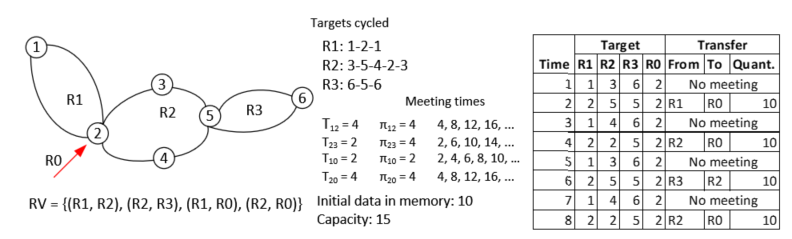
\includegraphics[scale=0.45]{Figures/KES_Figure3.png}
\caption{Synthetic example.}
\label{ex}
\end{figure}

\subsection{The proposed \emph{DynFloR} approach}\label{df}

For modeling the dynamic data collection process from the multi-robot network previously defined in Section \ref{tm}, we introduce a dynamic flow network based model which captures both the temporality of the patrolling process, as well as the dynamicity of the data collection and transfer. 

\subsubsection{The proposed dynamic network model}\label{model} 

Our proposed model adapts the dynamic network flow approach introduced in \cite{flow} by taking into account the specific requirements of multi-robot network patrolling. The flow network graph $G$ is constructed from moment 0 up to a moment of time $Time$. For each time step, the graph captures the state of each robot and the sink. Each of the states is represented by a node in the graph, which includes information such as robot decisions (data currently collected, data currently transferred, robot met for data exchange) or the amount of data stored. 

There are $(n+1) \cdot (Time+1) + 1$ \textbf{nodes} in the dynamic flow graph. For each robot $R_i$ including the sink ($\forall i, \; 0 \leq i \leq n$) there are $Time$+$1$ nodes, denoted by $i_t$ ($\forall t, \; 0 \leq t \leq Time$). The node $i_t$ corresponds to robot $R_i$ at time $t$. The \emph{sink} is viewed, in the proposed model, as robot $R_0$.  Besides the nodes corresponding to the robots, there is an additional \emph{source} node $s$ connected to all robots (except the sink) at time step 0.

The directed \textbf{edges} (connections) between the flow network's nodes and their capacities are set as follows. There is a connection between the source node $s$ and node $i_0$ ($\forall i, \;1 \leq i \leq n$) and its capacity is set to the the initial data $Q_i$ held by the robot $R_i$ at the beginning of the simulation. For each time moment $t$ when two robots $R_i$ and $R_j$ meet, two edges are added: one from $i_t$ to $j_t$ with capacity $\mathit{MaxCapacity_j}$ (i.e., the maximum memory of $R_j$) and one from $j_t$ to $i_t$ with capacity $\mathit{MaxCapacity_i}$ (i.e., the maximum memory of $R_i$). For each robot $R_i$ (including the sink) an edge is created between $i_t$ and $i_{t+1}$, $\forall t,\; 0 \leq t \leq Time-1$ (the edge has the capacity $\mathit{MaxCapacity_i}$). For each time moment $t$ when new data is collected by a robot $R_i$, an edge connecting the source node $s$ and the node $i_t$ is added and its capacity is set to $D_i$.      

We mention that the currently proposed model contains nodes corresponding to an entire cycle patrolled by a robot (without detailing the targets patrolled during each cycle). We also assume that a robot collects the data after it patrolled an entire cycle, this is why we add one edge with capacity $D_i$ after $k_i$ time units, instead of adding one edge with capacity $d_i$ to every node. The previous assumptions do not reduce the generality of $DynFloR$, as we can easily extend the model by adding new data at every time step to every robot and the $DynFloR$ algorithm remains the same. In this case, new data will be collected by a robot in a node corresponding to a target and not to an entire cycle (as in the current model).  

\subsubsection{$DynFloR$ algorithm}\label{dynflor}

After the flow network graph $G$ is built as described in Section \ref{model}, a maximum flow \cite{flow} from the source $s$ to the network sink (a node $0_t, t\leq Time$) will give the total amount of data that can be transferred to the base station in $t$ time steps.
Our proposal $\mathit{DynFloR}$ outputs the decision making strategy for each robot $R_i$, at each rendez-vous time, in order to increase the quantity of data received by the sink while respecting the memory constraint for each robot. 

The pseudocode for constructing the flow graph $G$ is presented in Algorithm \ref{alg:graph} and the $DynFloR$ algorithm is given in Algorithm \ref{alg:dynflor}. For determining the maximum flow in a graph $G$, the Preflow-Push algorithm \cite{Preflow} denoted by $getFlow$($G$) is used.  We also denoted by $addNode$ and $addEdge$ the operations for creating a node and an edge with a certain capacity, respectively. 

\begin{algorithm}[!htb]
\caption{Algorithm $DynFloR$}
    \label{alg:dynflor}
\begin{algorithmic}
\State{\textbf{Algorithm} $DynFloR$ is:}
\State{// determines the optimal policy for the robots' data delivery}
\Require{$n, k$ {\rmfamily - the number of robots and a list containing the robots' cycle lengths}
\\ \ \ \ {$D, Q, MaxCapacity$ \rmfamily - lists containing the amount of data collected by each robot, its initial data and its maximum memory}
\\ \ \ \ {$RV, Time$ \rmfamily - the list containing the pairs of robots that meet and the final moment of time considered}
\\ \ \ \ {$T, \pi$ \rmfamily - the initial meeting time for each pair of robots from $RV$ and their meeting period}
}
\Ensure{{\rmfamily returns the data delivery strategy for the robots from $RV$ (the path that gives the maximum flow in $G$)}}
\State{// read the input data}
\State{// construct the flow network graph $G$}
\State{$G \leftarrow CreateGraph$($n$,$k$,$D$,$Q$, $MaxCapacity$,$RV$,$Time$,$T$,$\pi$)}
\State{// the data delivery policy $Policy$ is computed from the path that corresponds to the maximum flow $MaxFlow$ in the graph $G$}
\State{$(MaxFlow, Policy) \leftarrow getFlow$($G$)}
\State{\textbf{EndAlgorithm} }
\end{algorithmic}
\end{algorithm}


\begin{algorithm}[!htb]
\caption{Function $CreateGraph$}
    \label{alg:graph}
\begin{algorithmic}
\Function{$CreateGraph$}{$n, k, D, Q, MaxCapacity,RV,Time,T,\pi$}
\State{// Create the flow network graph corresponding to the MRP problem}
\Require{$n, k, D, Q, MaxCapacity,RV,Time,T,\pi$ {\rmfamily the input parameters for the $DynFloR$ algorithm}}
\Ensure{returns the graph $G$ constructed as described in Section \ref{model}}
\State{// Create the nodes, edges and their capacities}
\State{$addNode$($G$,$s$) // a node corresponding to the source}
\For{$i \gets 0, n$}
\For{$t \gets 0, Time$}
\State{$addNode$($G$,$i_t$) // a node corresponding to robot $R_i$ at time $t$}
\If{$t \neq 0$}
\If{$i=0$}
\State{$addEdge$($G$,$i_{t-1}$,$i_t$,$\infty$)  // add an edge between $0_{t-1}$ and $0_t$ with capacity $\infty$}
\Else
%\State{// add an edge between $i_{t-1}$ and $i_t$ with capacity the memory of $R_i$}
\State{$addEdge$($G$,$i_{t-1}$,$i_t$,$MaxCapacity_i$) }
\EndIf
\EndIf
\EndFor
\If{$i \neq 0$} 
\State{$addEdge$($G$,$s$,$i_0$,$Q_i$)}% // add an edge between the source and $i_0$ with the  capacity of $D_i$}
\EndIf
\EndFor
\For{each pair $(i,j) \in RV$}
\For{$t \leftarrow T_{ij}, Time, \pi_{ij}$}
%\State{// add an edge corresponding to a possible transfer between $R_i$ and $R_j$ at time $t$}
\State{$addEdge$($G$,$i_t$,$j_t$,$MaxCapacity_i$)}
\If{$j \neq 0\;\;\;$} //if $j$ is not the sink 
%\State{// add an edge corresponding to a possible transfer between $R_j$ and $R_i$ at time $t$}
\State{$addEdge$($G$,$j_t$,$i_t$,$MaxCapacity_j$)} 
\EndIf
\EndFor
\EndFor
\State{// Add additional edges to model the data dynamically collected by the robots}
\For{$i \leftarrow 1, n$}
\For{$t \leftarrow 1, Time$}
\If{$t \;mod\; k_i=0\;\;$ // if an entire cycle was patrolled by robot $R_i$}
\State{// add an edge from the source to $i_t$ for modelling that new amount of data  $D_i$ arrives in the node}
\State{$addEdge$($G$,$s$,$i_t$,$D_i$)}
\EndIf
\EndFor
\EndFor
\State{// Return the graph $G$ }
\State{return $G$}
\EndFunction
\end{algorithmic}
\end{algorithm}

\noindent We note that the \emph{objective function} which has to be maximized in our approach is $$f(T)=\frac{data\;\;to\;\;sink\;\;until\;\;time\;\;T}{T}$$
Alternatively, we envisage the minimization of $$g(T) = \frac{input\;\; data\;\;-\;\;data\;\;to\;\;sink\;\;until\;\;time\;\;T}{T}$$

A brief analysis of the time complexity of $DynFloR$ is given below.  The time complexity of the $CreateGraph$ subalgorithm for constructing the dynamic network $G$ is $\mathcal{O}(|RV|\cdot Time)$. Therefore, the overall complexity of $DynFloR$, including computing the maximum flow, is $\mathcal{O}  \left( \mathcal{F}(n \cdot Time, |RV| \cdot Time) \right )$, where $\mathcal{F}(V, E)$ is the time complexity of a flow algorithm applied on a graph with $V$ nodes and $E$ edges (in our graph we have $n \cdot Time$ nodes and $|RV|\cdot Time$ directed edges). For example, for the highest label preflow-push algorithm \cite{Cormen:2009}, we have $\mathcal{F}=\mathcal{O} \left({(n \cdot Time)}^2 \cdot \sqrt{|RV|\cdot Time} \right)$. 



\subsection{Example}

For exemplifying how $DynFloR$ works, let us consider a very simple example of MRP illustrated in Figure \ref{ex:flow}. It consists of only two robots, denoted by R1 and R2. The sink is marked as R0. Figure \ref{ex:flow} also illustrates the first meeting time $T_{ij}$ between robots $i$ and $j$ and the meeting period $\pi_{ij}$ for robots $i$ and $j$. We are also assuming that the data collected by a robot is $15$, and the maximum memory $MaxCapacity_i$ for all robots is $55$. 

\begin{figure}[htb]
\centering
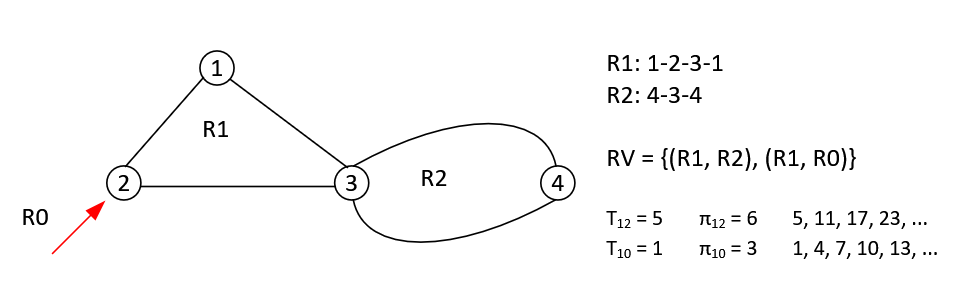
\includegraphics[scale=0.3]{Figures/SmallExaple.png}
\caption{Simple example.}
\label{ex:flow}
\end{figure}

For the MRP example from Figure \ref{ex:flow}, the associated flow network is presented in Figure \ref{patrolling}. In our example, the moment of time $T$ until the network is presented is 20. The amount of data which is collected by the robots is marked with green. \textcolor{black}{For a better readability of  Figure \ref{patrolling}}, we did not connect the green arrows to the source (as described in Section \ref{model}), but in the implementation they are connected. The decision making strategy for the robots, which is the output of the $DynFloR$ algorithm proposed in Section \ref{dynflor}, is marked with red. If an arc between two nodes $i_t$ and $j_t$ is labelled with a value $v$, it means that at time $t$ robot $R_i$ transfers to robot $R_j$ the amount $v$ of data. If the arc between $i_t$ and $i_{t+1}$ is labeled with $v$, it suggests that robot $R_i$ stores in its memory the amount of data $v$ for one unit of time (from $t$ to $t+1$).   

\begin{figure*}[!htb]
\centering
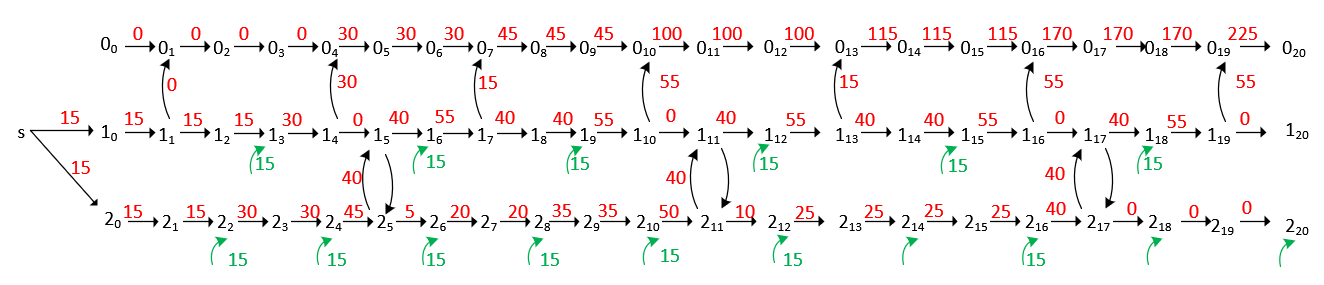
\includegraphics[scale=0.33]{Figures/FlowFinal2.png}

\caption{The dynamic network for the example from Figure \ref{ex:flow}. The decision making strategy for the robots is marked with red.}
\label{patrolling}
\end{figure*}

From Figure \ref{patrolling} we can observe that 225 units of data were transferred to the sink (robot R0) by $t = 20$. We can also observe that there are 3 green arrows (robot R2 at times 14, 18 and 20) that do not have incoming data. This data is not lost, it is stored in the memory of the robots, but since until the time limit we have set for the simulation ($t=20$) it cannot arrive to the sink, the flow algorithm does not consider it. But if we extended the time limit to include another meeting between robots R1 and R2, most of these data would arrive to the sink.

There is also the possibility to have lost data, a situation in which no matter how long we would extend the time limit, the data would never arrive to the sink. This is mainly due to the maximum memory capacity of the robots and the frequency of the collected data.    For instance, if we considered the value 40 as the maximum capacity for robot R2 (and left the other settings used for Figure \ref{patrolling} the same), by time 5, when R2 first meets R1 and has the chance to transfer data, it should have accumulated 45 units of data, which is impossible. In our model, if the robot's memory is full, the new data will not be collected (instead of overwriting existing data with the new one).

In order to determine which data is lost and which data is in the memory of a robot (and consequently will arrive to the sink in the future), we used the following method: after measuring the flow for time $Time$, as presented in Algorithm \ref{alg:dynflor}, we build a new, extended graph for time $2 \cdot Time$. In this extended graph we added the extra edges denoting new data coming from the source to the robots only until time step $Time$, so second half of the graph has no extra data coming. We measure the flow in this extended graph and the difference between the flows denotes the data that is in the memory of the robots at time $Time$ and will arrive to the sink later. We also know the total data that should enter the graph (the sum of the capacities of the outgoing arcs of the source node) and the difference between this data and the flow of the extended graph is the quantity of the data that is lost.
The robot that loses data is determined by the flow algorithm, and in the current implementation we only try to optimize the total quantity of data that arrives to the sink, and do not try to balance the lost quantities between robots.

\section{Results and discussion}\label{discussion}

In this section we present our current results obtained using the algorithm presented previously. The network flow part of our DynFloR algorithm was implemented using the Python NetworkX \cite{nx} graph library.

We performed incipient simulations on randomly generated inputs of $20$ robots with the same $MaxCapacity$ for each robot. Figures \ref{figure1} and \ref{figure2} show the evolution of the $f(T)$ and $g(T)$ objective functions for two different values of $MaxCapacity$. We observe that both functions converge to an equilibrium state and this convergence is independent of the memory capacity. Multiple random experiments confirm this.

\begin{figure*}[!htb]
\begin{minipage}{0.5\linewidth}
\centering
  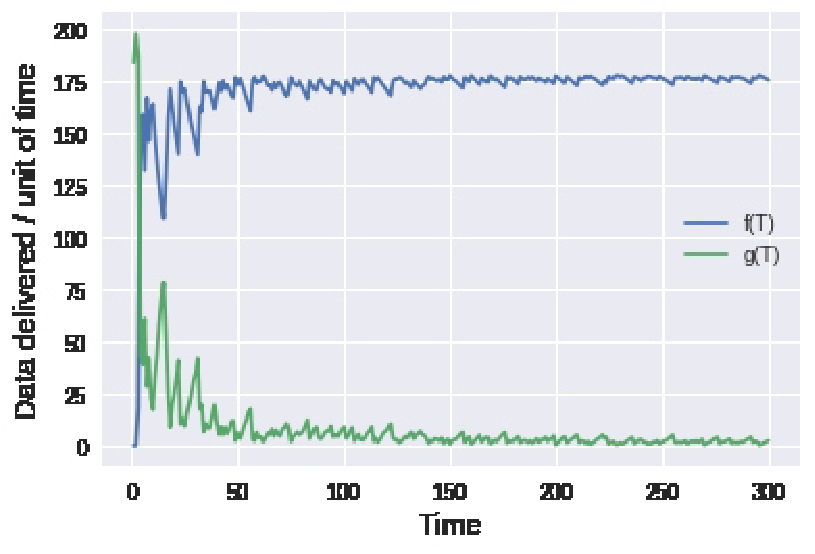
\includegraphics[scale=0.6]{Figures/graf1.pdf}
  \caption{Results for $20$ robots and $MaxCapacity=1000$. }
  \label{figure1}
\end{minipage}
\hfill
\begin{minipage}{0.5\linewidth}
\centering
  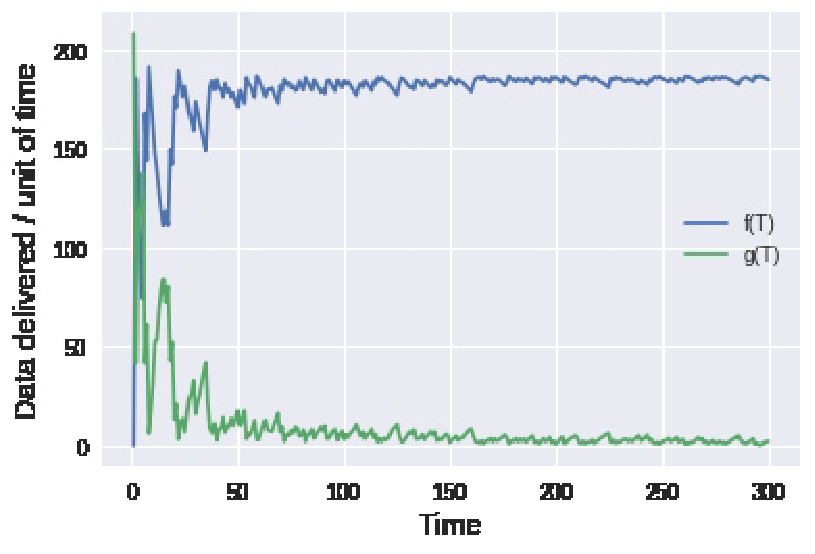
\includegraphics[scale=0.6]{Figures/graf2.pdf}
  \caption{Results for $20$ robots and $MaxCapacity=800$.}
  \label{figure2}
\end{minipage}
\end{figure*}

In order to better visualize the relation between data that enters the system, data that is currently in the memory of robots and data that is lost, we have performed some experiments using the simple example from Figure \ref{ex:flow}, setting the quantity of initial data and new data that is collected after every cycle to $15$. We have considered different values for $Time$ and $MaxCapacity$ (but considering the same capacity for both robots). The results are presented in Table \ref{table:memory}.

The value in parentheses after $Time$ represents the total quantity of data that enters the system until that time moment and which is divided into data that arrived to the sink, data that is currently in the memory of the robots, and data that is lost. We can see that as the $MaxCapacity$ of the robots increases, so does the amount that arrives to the sink and consequently the quantity of lost data decreases. From Table \ref{table:memory} it looks like setting the $MaxCapacity$ to 60 is enough to make sure that no data is lost, but in order to be certain of this, more experiments and maybe mathematical proof is necessary, because at time 20, there was no lost data for $MaxCapacity$ 55 either, but later this changed. Data that is currently in the memory of the robots is always bounded by the total memory the robots have, in our case $2 \cdot MaxCapacity$.

\begin{table}[!htb]
\small
\begin{center}
\resizebox{\textwidth}{!}{
\begin{tabular}{|c|c|c|c|c||c|c|c|c|c| } 
\hline
\textbf{Time} & \textbf{Maximum}  & \textbf{Data arrived} & \textbf{Data in} & \textbf{Lost} & \textbf{Time} & \textbf{Maximum}  & \textbf{Data arrived} & \textbf{Data in} & \textbf{Lost} \\
& \textbf{capacity} & \textbf{at sink} & \textbf{memory} & \textbf{data} & & \textbf{capacity} & \textbf{at sink} & \textbf{memory} & \textbf{data} \\
\hline \hline

\multirow{5}{*}{20 (270)} & 40 &  180   &  40  & 50  & \multirow{5}{*}{40 (420)} & 40 & 360    & 40 & 125        \\ \cline{2-5} \cline{7-10}

& 45 &   195& 45   & 30  &                     & 45 & 390     & 45    & 90        \\ \cline{2-5} \cline{7-10}

& 50 &  210& 45    & 15  &                   & 50 &     420 &  50     & 55       \\ \cline{2-5} \cline{7-10}

& 55 &  225    & 45 & 0  &                     & 55 &    450  & 55      & 20      \\ \cline{2-5}\cline{7-10}

& 60 &  240& 30   & 0    &                     & 60 &   480   & 45      &0       \\ \hline
\multirow{5}{*}{60 (705)} & 40 &  525   & 70  & 185  & \multirow{5}{*}{80 (1020)} & 40 & 730 & 40 & 250        \\ \cline{2-5} \cline{7-10}

& 45 & 570  & 75   & 135  &                     & 45 &     795 &45    &180         \\ \cline{2-5} \cline{7-10}

& 50 & 615&  80  & 85 &                   & 50 &    860 &   45   & 115      \\ \cline{2-5} \cline{7-10}

& 55 & 600 & 85& 35  &                     & 55 &   925  &  45   & 50      \\ \cline{2-5}\cline{7-10}

& 60 &  705 & 75  & 0  &                     & 60 &  990  & 30   & 0      \\ \hline
                    
 \end{tabular}}
  \caption{Quantity of data in memory, at the sink and lost, for different maximum capacities and time limits for the example from Figure \ref{ex:flow}. Initial data and new data received after every completed cycle is 15.  }
  \label{table:memory}
\end{center}
\end{table}

From Table \ref{table:memory} we can also observe that for a given $MaxCapacity$ the quantity of lost data is not double if we double $Time$. For example, for $MaxCapacity$ 50, we have 15 units of lost data after $Time$ 20, but if we double $Time$, the quantity of lost data becomes 55. We performed some experiments in order to better understand how the quantity of lost data changes if time increases, for a fixed $MaxCapacity$. In Table \ref{table:increase} we included two scenarios: the left part of the table was computed for $MaxCapacity$ 50, while the right part was computed for $MaxCapacity$ 40. For both scenarios, we computed also the rate of Lost data / Time (in the 4th and 8th column).

\begin{table}[!htb]
\small
\begin{center}
\resizebox{\textwidth}{!}{
\begin{tabular}{|c|c|c|c||c|c|c|c|} 
\hline
\textbf{Maximum}&\textbf{Time} & \textbf{Lost Data} & \textbf{Lost data / Time} & \textbf{Maximum}&\textbf{Time} & \textbf{Lost Data} & \textbf{Lost data / Time} \\
\textbf{capacity}&&&&\textbf{capacity}&&&\\
\hline \hline
&10 & 5    & 0.5 & &10 & 25 & 2.5\\ 
\cline{2-4}\cline{6-8}
&20 &  15  &  0.75& & 20 & 50 & 2.5\\ \cline{2-4}\cline{6-8}
&50 & 65    & 1.3 & & 50 & 150  & 3\\ \cline{2-4}\cline{6-8}
&100 &  155  & 1.55 & & 100 & 325 & 3.25\\ \cline{2-4}\cline{6-8}
&200& 315    &  1.575 & & 200 & 650 & 3.25\\ \cline{2-4}\cline{6-8}
&500& 815    &  1.63 & &500 & 1650 & 3.3\\ \cline{2-4}\cline{6-8}
50&1000& 1655   &  1.655& 40&1000 & 3325 & 3.325\\ \cline{2-4}\cline{6-8}
&5000 &  8315  & 1.663  & & 5000 & 16650 & 3.33\\ \cline{2-4}\cline{6-8}
&10000& 16655   &  1.6655& & 10000 &  33325& 3.3325\\ \cline{2-4}\cline{6-8}
&50000&  83315  & 1.6663 & &50000 &  166650 & 3.333\\ \cline{2-4}\cline{6-8}
&100000&   166655 & 1.66655  & &10000 &  333325 & 3.33325\\ \hline
\end{tabular}}
\caption{Progression of lost data as time increases for different $MaxCapacity$ values}
%50 (first three columns) and 40 (last three columns).}
\label{table:increase}
\end{center}
\end{table}

As expected, Table \ref{table:increase} reveals that the quantity of lost data per time significantly decreases as the maximum memory capacity of the robots increases. Additionally, as illustrated in Figure \ref{fig:lostdata}, it seems that the lost data per time converges to an equilibrium state, independent of the maximum capacity of the robots. This can be observed more clearly by running the proposed flow algorithm for more time steps, thus allowing all the data to arrive at the sink. As we have previously discussed, the data which does not arrive to the sink until a certain time limit is not necessarily lost, as it may arrive to the destination if we extend the time limit. Still, there is also the possibility to have lost data, a situation in which the data would never arrive to the sink no matter how long we would extend the time limit. Further experiments and theoretical analyses will be performed in this direction.

\begin{figure*}[!htb]
\centering
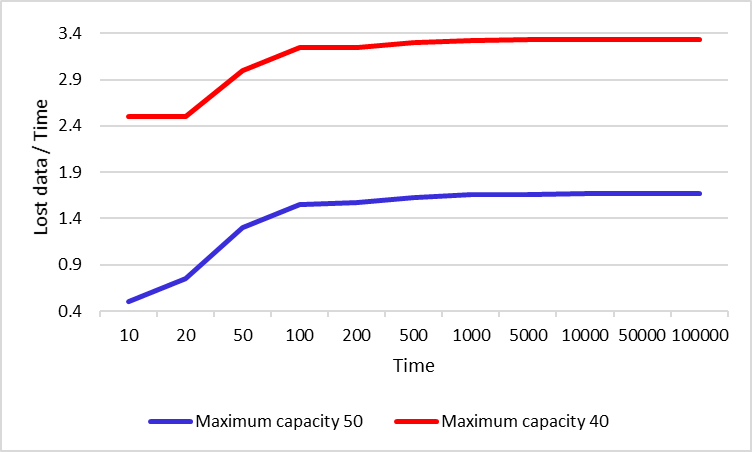
\includegraphics[scale=0.3]{Figures/Lost.png}
\caption{Variation of lost data per time for the example from Figure \ref{ex:flow}.}
\label{fig:lostdata}
\end{figure*}

\subsection{Comparison to related work}\label{compRelatedWordkDynFloR}

The literature contains various approaches related to multi-robot patrolling described in Section \ref{lr}, but we have not found approaches for optimizing data delivery in MRP.

Our work differs from the approaches described in Section \ref{lr}, as it has a different target than the previously described related work. It approaches the problem of data delivery optimization in a deterministic MRP setting using a dynamic flow based approach. As far as we know, approaches similar to $DynFloR$ do not exist in the MRP/DMRP literature. The most similar  approach to ours is the one of Liemhetcharat et al. \cite{Liemhetcharat2015}. The problem approached in the current chapter differs from the one of Liemhetcharat et al. \cite{Liemhetcharat2015}, even if both chapters are dealing with the data delivery problem. The perspectives are different, since the chapter \cite{Liemhetcharat2015} considers data delivery from a central location to several local targets, while in our chapter the perspective is the opposite one. 

A major advantage of $DynFloR$ is its polynomial time complexity, compared to the classical brute-force exponential solutions \cite{Romeo2018}. In addition, $DynFloR$ works well for dynamic data, i.e. data which continuously appear on each robot cycle. Another advantage of $DynFlor$ is that it finds the global optima, unlike the metaheuristic approaches (such as \emph{genetic algorithms} - GAs) \cite{portugal_2011}) which may provide a local optima. Besides, another difficulty when modelling the MRP using GAs relies on the chromosomes' modelling and on incorporating the continuous data collection into the model. An additional benefit of $DynFloR$ is that it can be adapted for the dynamic case of the MRP, under the same assumptions currently considered. When new targets are discovered during the dynamic patrolling problem and they are allocated to new patrolling robots, new nodes are simply added to the flow network graph $G$ and $DynFloR$ is executed again. An adaptive version of $DynFloR$ may be further investigated, with the goal of adapting the solution provided by $DynFloR$ instead of running it from scratch when new cycles to be patrolled are discovered.  

One of the current limitations of $DynFloR$ is given by the assumption regarding the periodicity of the robots' meetings. In the general case, in real DMRP scenarios,  instead of having initial meeting times and meeting periods, there is an uncertainty of the meetings as the robots' speed is not constant. For offering a solution to the data delivery optimization for the general case, \emph{reinforcement learning} would be further investigated  for adapting the robots'  decision making policy to the uncertainty of the world.  


\section{Conclusions and future work}\label{conc}

In this chapter we have investigated the data delivery optimization in a simplified setting  for the \emph{multi-robot patrolling} problem in which the environment is deterministic. We introduced accordingly a centralized and offline approach $DynFloR$ based on flows in dynamic networks. The goal of $DynFloR$ is to determine the robots' policy for maximizing  the quantity of data delivered to a base station in a given time, assuming that the robots are continuously collecting data during the patrolling. The more general aim of the research initiated in this chapter is to explore the general case of the problem  of optimizing the data delivery in DMRP when the environment is non-deterministic and uncertain (i.e. there are communication failures). 

Further work will extend the experimental evaluation and theoretical analysis of $DynFloR$ in order to better assess its performance. We also aim to decentralize the decision making process and to incorporate uncertainty in the communication between robots.  An extension of $DynFloR$ to an online approach and the incoming data model to an irregular one will be subjects to future developments. In order to achieve these goals, a \emph{reinforcement learning} perspective will be considered. 
